% DEX-Net — first draft (generated from paper/results; to be rewritten by the author).
% Numbers: every figure in this text comes from paper/results/final/, paper/results/economics/
% or the generated tables in paper/tables/. Comments marked CHECK flag statements the author
% should confirm or soften when rewriting.
\documentclass[11pt]{article}
\usepackage[margin=1in]{geometry}
\usepackage[T1]{fontenc}
\usepackage{lmodern}
\usepackage{amsmath,amssymb}
\usepackage{graphicx}
\usepackage{booktabs}
\usepackage{adjustbox}
\usepackage[numbers,sort&compress]{natbib}
\usepackage{xcolor}
\usepackage[colorlinks=true,linkcolor=blue!50!black,citecolor=blue!50!black,urlcolor=blue!50!black]{hyperref}
\graphicspath{{../figures/}}

\title{DEX-Net: Learning Only the Stochastic Part of\\ Uniswap v3 Order Flow}
\author{Clayton Barnes}
\date{Draft --- \today}

\begin{document}
\maketitle

\begin{abstract}
Liquidity providers in concentrated-liquidity automated market makers (AMMs) need simulators that reproduce how swaps, mints and burns arrive and interact, not only how prices move. We present DEX-Net, a pooled neural event model for Uniswap v3 that learns only the stochastic parts of order flow---event timing, event type, swap size relative to available depth, and liquidity ranges and amounts---and computes prices and liquidity exactly from pool state. Because the exact state is available during simulation, the model can also condition on the pool's liquidity profile around the current price. We train on 29.4 million events from ten Ethereum pools, with active liquidity reconciled exactly at every swap, and evaluate with three seeds per model on 1,217 fixed start points. On two pools held out from training, conditioning on the liquidity profile halves the 512-event energy score of an otherwise identical model (37.2 to 16.6), cuts spurious liquidity collapse from 24\% to 15\% of paths (real: 5\%), and brings the width of the simulated price distribution to 1.01 times the realised width (from 1.78). The liquidity-aware model is nonetheless slightly \emph{worse} at next-event likelihood, illustrating that one-step likelihood and simulation quality are different targets. The model beats a fitted multivariate Hawkes process on event timing and type, and matches or beats simple history-based forecasters on held-out pools. We document its failures: predicted skew is not directionally informative, swap-size tails remain too heavy, and just-in-time liquidity is too rare, too large relative to its deposit, and too often left in place. Finally, we measure what an LP simulator must get right: across ten pools on Ethereum, Arbitrum and Base, fees approximately equal loss-versus-rebalancing, and a perfect-foresight bound shows that the value of timing liquidity concentrates at intervals of minutes rather than days. We release code and a reconciled dataset.
\end{abstract}

% ===================================================================== 1
\section{Introduction}

A liquidity provider (LP) in a Uniswap v3 pool earns fees from swaps that trade through its price range and loses value to arbitrageurs who trade against stale pool prices. Both depend on the joint dynamics of order flow and liquidity: how often swaps arrive, how large they are relative to the liquidity they meet, and how other LPs add and remove liquidity around the price. Price-only simulators---geometric Brownian motion, GARCH-type models, or learned return generators---ignore this liquidity. Agent-based simulators represent it, but require behaviour to be specified by hand.

We take a third route. An AMM is a deterministic machine: given its state and an event, the next state follows exactly from the protocol's rules. What is uncertain is \emph{which} event arrives next---when, of which type, how large, and over which range. We learn only this stochastic part, from data, and compute everything else exactly. A simulated path is a sequence of sampled events, each applied to an exact replica of the pool.

This split has a second benefit that turns out to matter more than we expected. Because the simulator holds the exact pool state, the model can condition on quantities that a pure sequence model would have to infer, such as the liquidity available at each price level near the current price. Adding this liquidity profile as an input costs a little next-event likelihood but removes most of the model's long-horizon failures on pools it has never seen.

\paragraph{Contributions.}
\begin{enumerate}
\item A reconciled multi-pool Uniswap v3 event dataset: ten Ethereum pools from May 2021 to September 2026, with active liquidity reproduced exactly at every swap (Section~\ref{sec:data}).
\item DEX-Net, a pooled event model with exact, mechanics-consistent sampling and liquidity-profile conditioning (Section~\ref{sec:model}).
\item A multi-seed evaluation of next-event likelihood against point-process baselines, of rollouts against history-based forecasters, and of liquidity behaviour, with documented failure modes and evidence that likelihood and simulation quality diverge (Section~\ref{sec:results}).
\item An economic lens on what such simulators must capture: cross-chain measurements of fees against loss-versus-rebalancing, and a perfect-foresight bound on the value of timing (Section~\ref{sec:economics}).
\end{enumerate}

% ===================================================================== 2
\section{Background and related work}\label{sec:background}

\paragraph{Uniswap v3.} In Uniswap v3~\citep{adams2021uniswap}, LPs deposit liquidity $L$ over a price range $[p_a,p_b)$ expressed in discrete ticks. Within a tick interval the pool behaves as a constant-product market with \emph{active} liquidity equal to the sum of all positions covering the current price; a swap moves the price along this curve, crossing ticks and changing active liquidity as it goes. Mints and burns add and remove liquidity over ranges. Fees, a fixed fraction of swap input, accrue to in-range liquidity; since December 2025 a protocol share is withheld on mainnet pools.

\paragraph{LP economics.} Loss-versus-rebalancing (LVR)~\citep{milionis2022lvr} measures what an LP loses to arbitrageurs relative to a rebalancing strategy trading at external prices; with fees, the LP's excess return over that strategy is fees minus LVR~\citep{milionis2023fees}. Just-in-time (JIT) liquidity, in which an LP mints immediately before a large swap and burns immediately after, is a distinctive feature of v3 order flow~\citep{wan2022jit}. Impermanent loss in concentrated ranges is analysed by \citet{loesch2021impermanent}.

\paragraph{Temporal point processes.} Event sequences with marks are classically modelled by Hawkes processes~\citep{hawkes1971}; neural variants replace parametric intensities with recurrent~\citep{mei2017neuralhawkes} or attention-based~\citep{zuo2020transformerhawkes} encoders, or model inter-event times directly without an intensity~\citep{shchur2020intensityfree}. Our clock is in the last category, with a discrete-time (block) parameterisation.

\paragraph{Generative market simulators.} Limit-order-book simulators range from agent-based platforms such as ABIDES~\citep{byrd2020abides} to learned generators of order flow~\citep{coletta2021realistic,nagy2023lob}, typically evaluated against stylized facts of returns~\citep{cont2001stylized}. To our knowledge, learned generators of AMM order flow that keep the AMM's mechanics exact have not been studied. % CHECK: confirm with a literature search before claiming novelty.

% ===================================================================== 3
\section{Data}\label{sec:data}

\paragraph{Pools.} We use ten Ethereum Uniswap v3 pools: USDC, USDT, DAI and WBTC paired with WETH at the 0.05\% and 0.3\% fee tiers, and USDC/USDT at 0.01\% and 0.05\%. Pools were chosen by existence at a fixed roster block, not by current activity. The data cover May 2021 to September 2026 and include every Initialize, Swap, Mint and Burn log (Table~\ref{tab:dataset}): 29.4 million events, of which 28.24 million are swaps, 625,526 mints and 516,415 burns.

\begin{table}[t]
\centering
\small
\caption{Pools, event counts and chronological splits (model rows). Held-out pools contribute no training rows.}
\label{tab:dataset}
\begin{adjustbox}{max width=\linewidth}
\begin{tabular}{lllrrrrlrrr}
\toprule
Pool & Fee & Role & Events & Swaps & Mints & Burns & Dates & Train & Val & Test \\
\midrule
USDC/WETH & 0.05\% & fit & 12,064,159 & 11,652,190 & 219,779 & 192,190 & 2021-05-05 – 2026-09-15 & 8,416,528 & 1,833,866 & 1,813,701 \\
USDT/WETH & 0.05\% & fit & 7,064,516 & 6,965,286 & 52,348 & 46,882 & 2021-05-05 – 2026-09-15 & 4,746,323 & 1,139,022 & 1,179,107 \\
WBTC/WETH & 0.05\% & fit & 2,390,754 & 2,330,001 & 33,297 & 27,456 & 2021-05-05 – 2026-09-15 & 1,298,702 & 538,585 & 553,403 \\
DAI/WETH & 0.05\% & fit & 1,985,785 & 1,976,002 & 5,231 & 4,552 & 2021-05-05 – 2026-09-15 & 1,160,931 & 376,088 & 448,702 \\
USDC/USDT & 0.01\% & fit & 1,960,944 & 1,908,221 & 27,508 & 25,215 & 2021-11-13 – 2026-09-15 & 1,089,657 & 482,479 & 388,744 \\
USDT/WETH & 0.3\% & fit & 1,539,097 & 1,333,943 & 115,486 & 89,668 & 2021-05-05 – 2026-09-15 & 796,809 & 311,711 & 430,513 \\
USDC/WETH & 0.3\% & fit & 1,177,154 & 984,031 & 110,214 & 82,909 & 2021-05-04 – 2026-09-15 & 795,457 & 183,125 & 198,508 \\
DAI/WETH & 0.3\% & fit & 414,307 & 392,844 & 12,347 & 9,116 & 2021-05-04 – 2026-09-15 & 275,445 & 69,620 & 69,178 \\
WBTC/WETH & 0.3\% & held out & 479,419 & 404,556 & 42,471 & 32,392 & 2021-05-04 – 2026-09-15 & — & 88,503 & 66,414 \\
USDC/USDT & 0.05\% & held out & 305,855 & 292,975 & 6,845 & 6,035 & 2021-05-04 – 2026-09-15 & — & 16,849 & 18,163 \\
\midrule
Total &  &  & 29,381,990 & 28,240,049 & 625,526 & 516,415 &  &  &  &  \\
\bottomrule
\end{tabular}
\end{adjustbox}
\end{table}


\paragraph{Reconciliation.} We replay every pool from its first event with exact integer arithmetic. A Fenwick-tree ledger of liquidity by tick reproduces the active liquidity recorded by the contract at every one of the 28.24 million swaps; the block-header hash chain is checked; owner and range balances never go negative; and all 516,415 burns are confirmed to remove liquidity that exists. The same ledger provides the exact state at any point for simulation.

\paragraph{Representation.} Each pool is expressed in an economic base/quote orientation (e.g.\ WETH priced in USDC). Swap sizes are measured relative to the pool's virtual base reserve, liquidity amounts relative to active liquidity, and ranges relative to the current tick in units of tick spacing. Each event is summarised by twelve features with validity masks. Pool metadata (fee tier, tick spacing and token decimals) enters as five features.

\paragraph{Liquidity profile.} For every event we also record the liquidity profile just before it: the active liquidity at 17 log-price offsets between $-4\%$ and $+4\%$ of the current price, as $\log(1+L(\text{offset})/L(\text{now}))/4$. During training the profile is read from the reconciled ledger; during simulation it is recomputed from the simulated book after every event. The two computations agree exactly on real data.

\paragraph{Splits.} Splits are chronological by block: training until 2 February 2025, validation until 14 November 2025, and test until 15 September 2026. Eight pools are used for fitting; WBTC/WETH 0.3\% and USDC/USDT 0.05\% are held out entirely and contribute validation and test data only. All scalers are fitted on training rows.

% ===================================================================== 4
\section{Model}\label{sec:model}

Figure~\ref{fig:architecture} summarises the model and the sampling loop.

\begin{figure}[t]
\centering
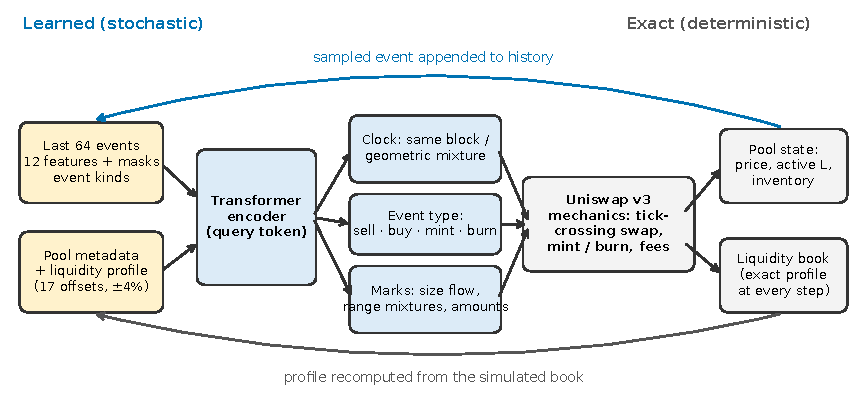
\includegraphics[width=\linewidth]{fig1_architecture.pdf}
\caption{DEX-Net. A Transformer encoder reads the last 64 events, pool metadata and (in the depth-aware model) the liquidity profile, and parameterises distributions over the next event's timing, type and marks. A sampled event is applied by exact Uniswap v3 mechanics; the resulting state yields the next liquidity profile and the event joins the history.}
\label{fig:architecture}
\end{figure}

\paragraph{Event space.} The next event is a sell, buy, mint or burn, arriving after a gap of $d\in\{0,1,2,\dots\}$ blocks, where $d=0$ means the same block as the previous event.

\paragraph{Clock.} A logit gives the probability of another event in the same block; otherwise the gap $d\geq1$ follows a three-component geometric mixture, $P(d)=\sum_k \pi_k(1-e^{-r_k})e^{-(d-1)r_k}$, with mixture weights and rates output by the network.

\paragraph{Type and marks.} The event type is a four-way categorical conditioned on the gap. Marks are conditioned on gap and type:
\begin{itemize}
\item \emph{Swap size}: a rational-quadratic spline flow~\citep{durkan2019spline} on the log of the base amount relative to the virtual base reserve. Buys are truncated at the exact amount the pool's liquidity can supply.
\item \emph{Mint range}: discretized logistic mixtures~\citep{salimans2017pixelcnnpp} over the lower tick (relative to the current tick, on an asinh scale) and the width (log scale), on the pool's tick grid. Interval endpoints are computed in double precision: in single precision, far from the current tick, the two edges of a one-tick interval can round to the same number.
\item \emph{Mint amount}: a spline flow on $\log(L/L_{\text{active}})$.
\item \emph{Burn}: the same range model, normalised over the ranges that actually hold liquidity, followed by a full-burn indicator and a spline flow for partial fractions.
\end{itemize}

\paragraph{Encoder.} A Transformer~\citep{vaswani2017attention} reads the last 64 events (features, masks and event-type embeddings) and a query token carrying pool metadata. In the depth-aware model the liquidity profile is projected and added to the query token. The headline model has width 128 and 4 layers (956,527 parameters); the reference model is identical without the profile (954,351); a small depth-aware model has width 64 and 2 layers (148,975).

\paragraph{Exact simulation.} To simulate, we sample an event, apply it to the replicated pool with exact tick-crossing swap arithmetic or exact liquidity updates, compute its features from the before and after states, and append it to the history. A sampled event that is infeasible (for example, a burn of liquidity that does not exist) ends the path and is recorded as a failure; it is never repaired.

\paragraph{Training.} We minimise next-event negative log-likelihood (NLL), the sum of the clock, type and mark terms, with AdamW~\citep{loshchilov2019adamw} (learning rate $10^{-4}$, weight decay 0.01, 1,000-update warm-up then cosine decay to 10\%, gradient clipping at 1), batches of 1,024 events, and a pool-balanced schedule covering each fitting pool's training rows three times (202 million examples). Validation NLL on 8,192 fixed rows per seen pool is computed after each of 97 rounds, and the checkpoint with the lowest seen-pool macro NLL is kept; there is no early stopping. Each of the 15 final runs took 11--14 hours, with three or four runs sharing each of four A100 GPUs.

% ===================================================================== 5
\section{Evaluation setup}\label{sec:setup}

\paragraph{Model families.} We train five families with three seeds each (260930--260932), all with identical code, schedules (one per seed, shared across families) and hardware: the reference model; the depth-aware model; the small depth-aware model; and two history ablations of the depth-aware model that see only the last 8 events or no events at all.

\paragraph{Next-event likelihood.} NLL is reported in nats per event on 32,768 fixed rows per pool from the test period, as a macro average over seen pools and over held-out pools.

\paragraph{Point-process baselines.} For the clock and type terms we fit two baselines by maximum likelihood on the same event space, scored on the same rows: an \emph{unconditional} renewal model (constant same-block probability, a three-component geometric mixture for gaps, constant type frequencies), and a four-type discrete-time \emph{Hawkes} process~\citep{hawkes1971} over the same last 64 events, with exponential kernels at two learned time scales, a closed-form per-block hazard for gaps, and type probabilities proportional to type intensities. Both are fitted per seen pool; held-out pools use one fit on pooled seen-pool data.

\paragraph{Rollouts.} Start points (\emph{anchors}) are spaced uniformly in event index within each split, never chosen by outcome, with non-overlapping outcome windows; at each we reconstruct the exact pool state and position inventory from the raw logs. There are 610 test anchors (512 in seen pools, 98 in held-out pools) and 607 validation anchors (512 and 95). Each model seed draws 32 paths per anchor. At 32, 128 and 512 events we score four endpoints---price return (bp), log change in active liquidity, elapsed blocks and traded volume relative to the initial reserve---with the energy score~\citep{gneiting2007scoring}, an unbiased ensemble estimator on scaled endpoints, and report price CRPS where useful. Model families are compared by paired bootstrap over anchors.

\paragraph{History-based forecasters.} Each anchor also carries two baselines built from the pool's own history, scored identically: \emph{recent}, 256 endpoint windows of the same length drawn from the events just before the anchor; and \emph{expanding}, 256 windows drawn from all prior history.

% ===================================================================== 6
\section{Results}\label{sec:results}

\subsection{Next-event likelihood}

Table~\ref{tab:nll_by_pool} reports NLL by pool. The reference model is best on aggregate (seen 5.534, held-out 7.649); the depth-aware model is marginally worse (+0.008 seen, s.e.\ 0.004; +0.018 held-out, s.e.\ 0.011). The small model costs +0.08 and +0.13. History matters a great deal: with only the last eight events the depth-aware model loses 0.18 nats per event on seen pools and 0.29 on held-out pools, far beyond seed-to-seed variation; with no history it loses 1.04 on seen pools.

The no-history model fails on held-out pools (23.6 $\pm$ 9.8). The failure is concentrated in one component and one pool: event timing in USDC/USDT 0.05\%, where the clock NLL reaches 12--47 nats instead of 1--2. Without history the model cannot tell how active an unseen pool is. Its validation NLL is also lowest after very few training rounds (rounds 2, 3 and 16 of 97 across seeds), after which it learns the training period's average activity at the expense of transfer to later periods.

\begin{table}[t]
\centering
\small
\caption{Next-event NLL (nats/event) on the test period, mean $\pm$ s.d. over 3 seeds; 32,768 fixed examples per pool.}
\label{tab:nll_by_pool}
\begin{adjustbox}{max width=\linewidth}
\begin{tabular}{lrrrrr}
\toprule
Pool & Reference & Depth-aware & Depth 64$\times$2 & Depth, 8 events & Depth, no history \\
\midrule
USDC/WETH 0.05\% & 4.775 $\pm$ 0.006 & 4.792 $\pm$ 0.005 & 4.887 $\pm$ 0.009 & 4.974 $\pm$ 0.006 & 5.476 $\pm$ 0.030 \\
USDT/WETH 0.05\% & 4.454 $\pm$ 0.009 & 4.461 $\pm$ 0.003 & 4.584 $\pm$ 0.005 & 4.640 $\pm$ 0.008 & 5.125 $\pm$ 0.007 \\
WBTC/WETH 0.05\% & 4.988 $\pm$ 0.009 & 4.998 $\pm$ 0.007 & 5.099 $\pm$ 0.051 & 5.115 $\pm$ 0.012 & 6.047 $\pm$ 0.046 \\
DAI/WETH 0.05\% & 4.704 $\pm$ 0.004 & 4.715 $\pm$ 0.002 & 4.823 $\pm$ 0.009 & 4.895 $\pm$ 0.005 & 5.506 $\pm$ 0.052 \\
USDC/USDT 0.01\% & 5.904 $\pm$ 0.003 & 5.902 $\pm$ 0.001 & 5.952 $\pm$ 0.008 & 6.030 $\pm$ 0.006 & 6.531 $\pm$ 0.091 \\
USDT/WETH 0.3\% & 7.244 $\pm$ 0.027 & 7.260 $\pm$ 0.039 & 7.310 $\pm$ 0.039 & 7.564 $\pm$ 0.029 & 9.204 $\pm$ 0.063 \\
USDC/WETH 0.3\% & 6.598 $\pm$ 0.012 & 6.603 $\pm$ 0.009 & 6.623 $\pm$ 0.011 & 6.839 $\pm$ 0.009 & 8.083 $\pm$ 0.035 \\
DAI/WETH 0.3\% & 5.602 $\pm$ 0.005 & 5.606 $\pm$ 0.006 & 5.684 $\pm$ 0.002 & 5.720 $\pm$ 0.003 & 6.696 $\pm$ 0.083 \\
WBTC/WETH 0.3\% (held out) & 7.070 $\pm$ 0.022 & 7.075 $\pm$ 0.027 & 7.206 $\pm$ 0.031 & 7.274 $\pm$ 0.009 & 8.723 $\pm$ 0.041 \\
USDC/USDT 0.05\% (held out) & 8.228 $\pm$ 0.018 & 8.259 $\pm$ 0.041 & 8.389 $\pm$ 0.031 & 8.631 $\pm$ 0.093 & 38.377 $\pm$ 19.626 \\
\midrule
Macro, seen pools & 5.534 $\pm$ 0.005 & 5.542 $\pm$ 0.005 & 5.620 $\pm$ 0.010 & 5.722 $\pm$ 0.004 & 6.583 $\pm$ 0.024 \\
Macro, held-out pools & 7.649 $\pm$ 0.003 & 7.667 $\pm$ 0.019 & 7.797 $\pm$ 0.028 & 7.953 $\pm$ 0.046 & 23.550 $\pm$ 9.794 \\
\bottomrule
\end{tabular}
\end{adjustbox}
\end{table}


Table~\ref{tab:point_process_baselines} compares the clock and type terms with the point-process baselines. A converged Hawkes fit improves on the unconditional baseline substantially (3.50 to 3.23 nats on seen pools, 7.25 to 5.52 on held-out pools), and the neural model improves on Hawkes by a further 0.14 and 0.39. Most of the gain is in event type (0.67 against 0.74 on seen pools) and, on held-out pools, in timing (4.45 against 4.73). Marks have no point-process analogue; the no-history ablation is the corresponding comparison for them.

\begin{table}[t]
\centering
\small
\caption{Clock and event-type NLL (nats/event, macro over pools) on the same evaluation rows. Point-process baselines are fitted per seen pool; held-out pools use one fit on pooled seen-pool data. Neural rows are 3-seed means.}
\label{tab:point_process_baselines}
\begin{adjustbox}{max width=\linewidth}
\begin{tabular}{lrrrrrr}
\toprule
Model & Clock (seen) & Type (seen) & Sum (seen) & Clock (held out) & Type (held out) & Sum (held out) \\
\midrule
Unconditional (renewal + type frequencies) & 2.606 & 0.896 & 3.503 & 6.285 & 0.964 & 7.250 \\
4-type Hawkes, 2 time scales & 2.495 & 0.736 & 3.231 & 4.730 & 0.784 & 5.515 \\
DEX-Net & 2.422 & 0.669 & 3.091 & 4.456 & 0.668 & 5.124 \\
No profile (neural) & 2.421 & 0.667 & 3.088 & 4.451 & 0.667 & 5.119 \\
\bottomrule
\end{tabular}
\end{adjustbox}
\end{table}


\subsection{Rollouts}

Figure~\ref{fig:cones} shows forecast cones at four randomly drawn test anchors, and Table~\ref{tab:rollout_energy} reports energy scores for all models and baselines.

\begin{figure}[t]
\centering
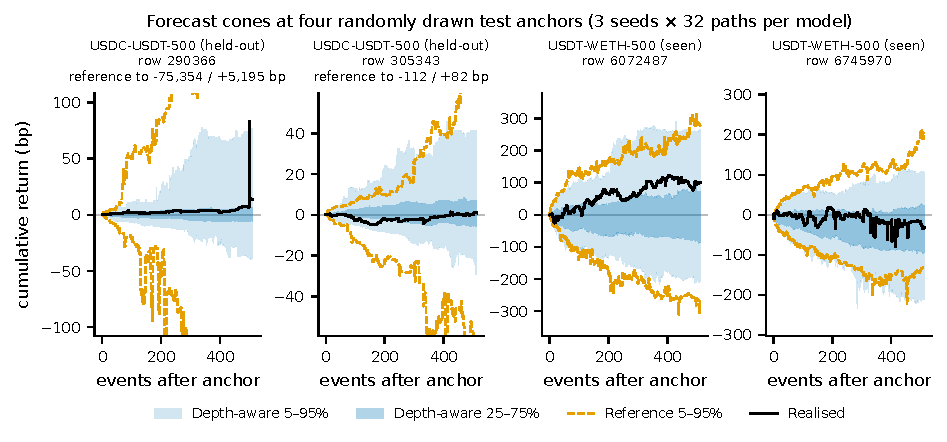
\includegraphics[width=\linewidth]{fig2_forecast_cones.pdf}
\caption{Forecast cones of cumulative return at four test anchors drawn at random (two held-out, two seen), from 96 paths per model (3 seeds $\times$ 32). Axes are scaled to the depth-aware model and the realised path; where the reference model's 5--95\% band leaves the axis its extent is printed in the panel title.}
\label{fig:cones}
\end{figure}

\begin{table}[t]
\centering
\small
\caption{Rollout energy score (lower is better) at 32/128/512 events, on the anchors where every path of every model reached the horizon (the same anchors in every column); models are the mean of 3 seeds $\times$ 32 paths; best per row in bold.}
\label{tab:rollout_energy}
\begin{adjustbox}{max width=\linewidth}
\begin{tabular}{lllrrrrrr}
\toprule
Period & Pools & Events & Anchors & Reference & Depth-aware & Depth 64$\times$2 & Recent & Expanding \\
\midrule
Test & held out & 32 & 97 & 3.45 & \textbf{2.77} & 3.03 & 3.17 & 3.62 \\
Test & held out & 128 & 95 & 8.81 & \textbf{6.27} & 6.31 & 6.49 & 7.24 \\
Test & held out & 512 & 79 & 36.60 & \textbf{18.48} & 18.55 & 19.37 & 19.82 \\
\midrule
Test & seen & 32 & 511 & 3.01 & \textbf{3.00} & 3.01 & 3.58 & 4.10 \\
Test & seen & 128 & 509 & \textbf{7.82} & 7.86 & 8.20 & 8.00 & 10.80 \\
Test & seen & 512 & 500 & 26.04 & 25.59 & 30.90 & \textbf{21.70} & 32.68 \\
\midrule
Validation & held out & 32 & 95 & 7.24 & 6.64 & \textbf{6.24} & 6.93 & 7.28 \\
Validation & held out & 128 & 92 & 15.97 & 12.14 & 11.55 & \textbf{11.42} & 13.33 \\
Validation & held out & 512 & 77 & 56.30 & 36.94 & \textbf{36.80} & 37.89 & 40.69 \\
\midrule
Validation & seen & 32 & 512 & 5.33 & \textbf{5.30} & 5.35 & 6.22 & 6.51 \\
Validation & seen & 128 & 510 & 12.24 & \textbf{12.12} & 12.48 & 14.36 & 15.29 \\
Validation & seen & 512 & 505 & 38.22 & \textbf{36.85} & 40.17 & 43.23 & 44.70 \\
\bottomrule
\end{tabular}
\end{adjustbox}
\end{table}


\paragraph{Held-out pools.} Here the liquidity profile changes the picture. In the test period the depth-aware model's 512-event energy is 16.55 against 37.24 for the reference model, a paired difference of $-18.5$ (95\% CI $-27.3$ to $-10.8$); the validation period shows the same ($-19.4$, CI $-36.6$ to $-5.6$), and in the test period the improvement is significant at every horizon (Table~\ref{tab:depth_vs_reference}). In the test period a depth-aware model (the 128$\times$4 model, or the 64$\times$2 model at 128 events) is the best forecaster at every horizon, slightly ahead of the recent-history baseline. In the validation period the recent baseline is ahead by 6.5\% at 128 events and 5\% at 512. We therefore describe the model as matching the strongest simple forecaster on unseen pools, while avoiding the reference model's failure.

\paragraph{Seen pools.} On seen pools the two 128$\times$4 models are close, with the depth-aware model ahead at 512 events in validation ($-1.34$, CI $-2.59$ to $-0.17$). In the validation period it beats both history baselines at every horizon (512 events: 37.95 against 44.16 for the recent baseline). In the test period, however, the recent baseline wins at 512 events (21.93 against 25.71). % CHECK: the test period includes the December 2025 protocol-fee switch; whether this shift explains the gap is untested.

\paragraph{Capacity.} The small depth-aware model matches the large one on held-out pools but is clearly worse on seen pools at long horizons (+5.3 at 512 events, CI 4.4 to 6.4).

\begin{table}[t]
\centering
\small
\caption{Depth-aware minus reference: paired energy difference with 95\% bootstrap CI over the Table 4 anchors; share of paths losing >63\% of active liquidity; 5–95\% return-spread ratio (simulated / realised).}
\label{tab:depth_vs_reference}
\begin{adjustbox}{max width=\linewidth}
\begin{tabular}{lllrrrrrr}
\toprule
Period & Pools & Events & Δ energy [95\% CI] & Collapse real & Collapse ref. & Collapse depth & Spread ref. & Spread depth \\
\midrule
test & seen & 32 & -0.00 [-0.04, +0.04] & 1.0\% & 0.8\% & 0.8\% & 1.06$\times$ & 1.08$\times$ \\
test & seen & 128 & +0.04 [-0.07, +0.15] & 1.2\% & 1.6\% & 1.6\% & 1.24$\times$ & 1.25$\times$ \\
test & seen & 512 & -0.45 [-1.10, +0.23] & 1.6\% & 3.9\% & 3.1\% & 1.46$\times$ & 1.37$\times$ \\
test & held out & 32 & -0.68 [-1.56, -0.10] & 3.1\% & 5.2\% & 4.0\% & 1.07$\times$ & 0.95$\times$ \\
test & held out & 128 & -2.55 [-4.46, -1.09] & 2.0\% & 13.0\% & 8.3\% & 1.29$\times$ & 1.05$\times$ \\
test & held out & 512 & -18.11 [-27.09, -10.48] & 5.1\% & 24.2\% & 15.2\% & 1.78$\times$ & 1.01$\times$ \\
val & seen & 32 & -0.03 [-0.08, +0.02] & 2.0\% & 2.3\% & 2.3\% & 1.16$\times$ & 1.17$\times$ \\
val & seen & 128 & -0.12 [-0.35, +0.07] & 3.1\% & 3.3\% & 3.2\% & 1.02$\times$ & 1.02$\times$ \\
val & seen & 512 & -1.37 [-2.65, -0.24] & 3.5\% & 6.8\% & 6.0\% & 1.21$\times$ & 1.12$\times$ \\
val & held out & 32 & -0.60 [-1.71, +0.02] & 4.2\% & 5.7\% & 4.6\% & 1.01$\times$ & 0.93$\times$ \\
val & held out & 128 & -3.83 [-8.25, -1.01] & 4.2\% & 14.8\% & 9.5\% & 1.13$\times$ & 0.99$\times$ \\
val & held out & 512 & -19.36 [-36.53, -5.49] & 8.4\% & 30.6\% & 19.9\% & 1.77$\times$ & 0.80$\times$ \\
\bottomrule
\end{tabular}
\end{adjustbox}
\end{table}


\paragraph{Path reweighting.} A post-hoc reweighting of simulated paths, fitted only on seen-pool validation rollouts (a bounded weight per path from its endpoints relative to its ensemble, with a penalty on divergence from uniform weights), improves the depth-aware model's 512-event energy by 1.65 on seen pools (CI 1.19 to 2.18) and 1.92 on held-out pools (CI 0.92 to 3.23). Reweighted, the model is ahead of the recent baseline on held-out pools at 512 events (17.35 against 17.57) but not on seen pools (27.2 against 22.6). Reweighting changes only weights, not paths, and we treat it as an optional calibration layer rather than part of the model. % Note: reweight-depth.json scores the finite weighted distribution with a V-statistic, so its absolute values differ from Table 4; compare within that file only.

\subsection{Liquidity behaviour}

\paragraph{Liquidity collapse and swap-size tails.} The reference model's long-horizon failures on held-out pools come from paths in which simulated liquidity thins and then collapses. One-step swap sizes are close to calibrated (for example, the predicted share of swaps larger than 1\% of the virtual reserve is 0.043\% against 0.038\% observed on seen test pools); the error is state-dependent. Once a path's active liquidity is low, swaps sized relative to the virtual reserve move the price far more, which thins liquidity further. On held-out pools, 24.2\% of the reference model's paths lose more than 63\% of their active liquidity within 512 events, against 5.1\% of real outcomes; the depth-aware model reduces this to 15.2\%. Swaps that move the price by more than 100 bp make up 0.97\% of the reference model's simulated swaps on held-out pools, 0.20\% of the depth-aware model's, and 0.03\% of real swaps; for moves above 500 bp the shares are 0.48\%, 0.066\% and 0.018\%. The liquidity profile removes most of the excess, but not all of it.

\paragraph{Just-in-time liquidity.} We apply the definitions of an earlier study in our research code to simulated paths and to the real test-period event stream identically (Figure~\ref{fig:jit}). A strict JIT pair is a mint, swap and burn that are consecutive, in one block, and share the same range and liquidity amount; a large mint adds more than ten times the active liquidity. The model learns the pattern: it generates strict JIT pairs, and its share of large mints is close to real (seen pools: 7.5\% of mints against 9.0\%). But JIT is too rare (1.8 pairs per 1,000 events against 4.6 on seen pools; 1.2 against 6.4 on held-out pools), too large relative to the deposit (median swap of 0.74\% of the deposit against 0.12\%), and too sticky (10.5\% of large mints are not removed within 64 events, against 0.5\%). Liquidity conditioning helps with the last of these (the reference model leaves 15.2\% unremoved).

\begin{figure}[t]
\centering
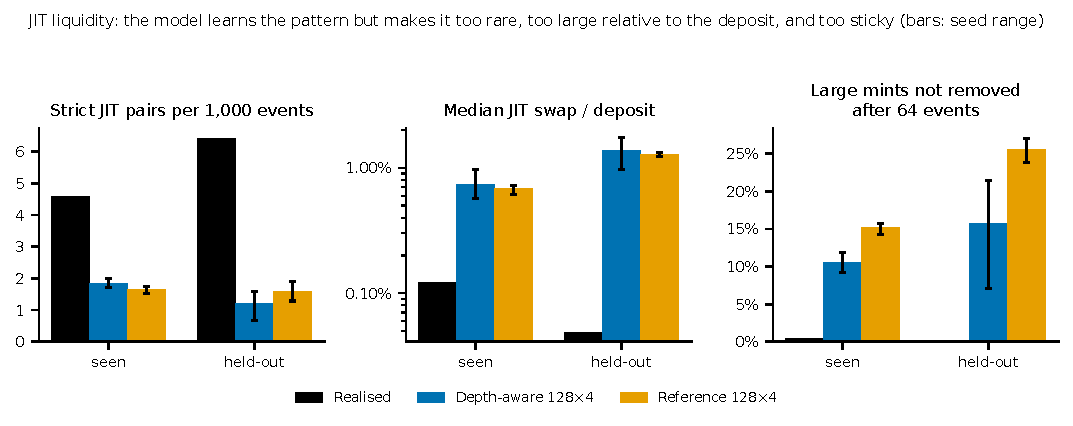
\includegraphics[width=\linewidth]{fig4_jit.pdf}
\caption{JIT liquidity, real against the final models, on seen and held-out pools: strict JIT pairs per 1,000 events, median ratio of the paired swap's notional to the minted deposit (log scale), and the share of large mints not removed within 64 events. Bars are seed means; whiskers show the range over three seeds. Simulated: 12 test anchors per pool, 32 paths of 96 events per seed. Real: the full test-period event stream.}
\label{fig:jit}
\end{figure}

\subsection{Stylized facts, calibration and skew}

Figure~\ref{fig:stylized} compares simulated and realised event sequences. The event mix is close; the same-block share is slightly low on seen pools (0.18 against 0.23). On seen pools the width of the simulated return distribution is within about 12\% of realised up to 32 events and widens to about 1.4 times realised at 512 events. On held-out pools, the depth-aware model stays within roughly 0.9--1.3 times realised at every horizon, while the reference model reaches about 5 times at 512 events. Volatility clustering is too strong in every model: the autocorrelation of absolute per-event returns exceeds the realised value at every lag (seen pools, lag 1: 0.21 against 0.17). PIT histograms (Figure~\ref{fig:pit}, Appendix) show no gross miscalibration of the return forecast but visible deviations at individual horizons.

\begin{figure}[t]
\centering
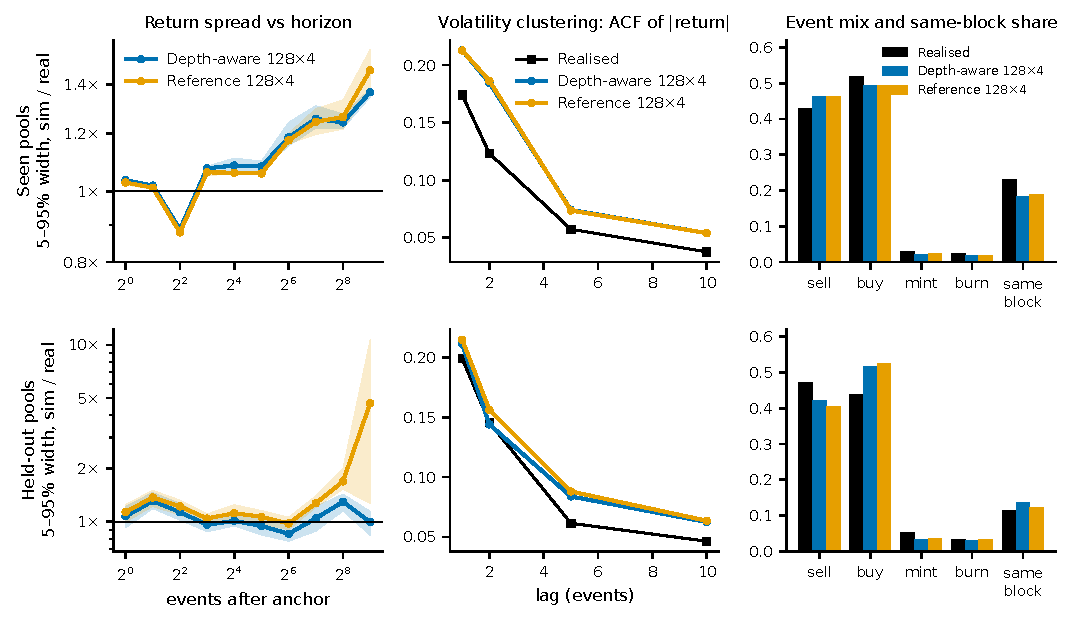
\includegraphics[width=\linewidth]{fig3_stylized_facts.pdf}
\caption{Stylized facts after test anchors, seen (top) and held-out (bottom) pools. Left: width of the 5--95\% range of cumulative return, simulated over realised, by horizon (shaded: seed range). Centre: autocorrelation of absolute per-event return. Right: event mix and same-block share.}
\label{fig:stylized}
\end{figure}

Predicted asymmetry is not directionally informative. We measure skew as the quantile skew of the forecast return, estimated from different paths from those used to set the tail thresholds to avoid a spurious negative relation. The correlation between predicted skew and realised tail asymmetry lies between $-0.12$ and $0.00$ at every horizon and pool group, with every confidence interval including zero. Restricting attention to the 20\% of anchors where the model is most confident does not help. On held-out pools, anchors with the most negative predicted skew were followed by upside breakouts 65--86\% of the time (19 anchors per group; small samples). Predicted skew follows the preceding trend (correlation 0.07--0.20 between the prior move and predicted skew), but realised outcomes after strong trends show no consistent direction, so this carried-over momentum is not rewarded.

\subsection{Likelihood is not simulation quality}\label{sec:nll-vs-sim}

Figure~\ref{fig:nllsim} places each model family by next-event NLL and 512-event energy. On held-out pools the ordering by likelihood is reversed: the reference model has the best NLL but by far the worst rollouts, and the small depth-aware model has much worse NLL than the reference model but rollouts as good as the large depth-aware model. The failures that matter for simulation are rare and state-dependent---thin liquidity, oversized swaps in a depleted book---so they carry little weight in an average one-step likelihood but compound over a rollout. Model selection for simulators should therefore use rollout scores, or at least check them.

\begin{figure}[t]
\centering
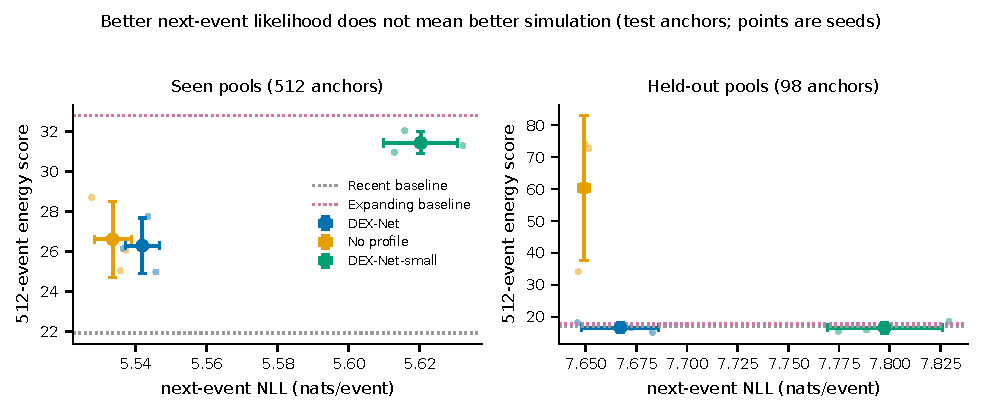
\includegraphics[width=\linewidth]{fig5_nll_vs_rollout.pdf}
\caption{Next-event NLL against 512-event energy on test anchors for the three rollout-evaluated families; large points are seed means with standard deviations, small points are individual seeds; dotted lines are the history-based forecasters.}
\label{fig:nllsim}
\end{figure}

% ===================================================================== 7
\section{An economic lens: what must an LP simulator get right?}\label{sec:economics}

\paragraph{Fees against LVR.} For marginal in-range liquidity, an LP's excess return over a rebalancing strategy is fees minus LVR, which we measure swap by swap against Binance ETH/USDT one-second prices. On synthetic pools the measurement recovers the theoretical $\sigma^2/8$ rate. We apply it to the four WETH/stablecoin pools on Ethereum and to the six WETH/USDC pools on Arbitrum and Base, using 61 million swaps that we verified against on-chain price checkpoints, over 380 common days from September 2025 (Figure~\ref{fig:fees}). Fees approximately equal LVR: excluding the 0.01\% pools, the ratio ranges from 0.77 (Ethereum USDC/WETH 0.05\%) to 1.06 (Base 0.3\%); the 0.01\% pools on Arbitrum and Base are at 0.47 and 0.81. LVR itself is similar everywhere, around 1.3--1.5 bp per day for marginal in-range liquidity, consistent with competition pushing fees towards LVR. A passive in-range LP therefore earns roughly nothing over rebalancing, and any value must come from \emph{when} liquidity is provided.

\begin{figure}[t]
\centering
\begin{minipage}{.49\linewidth}\centering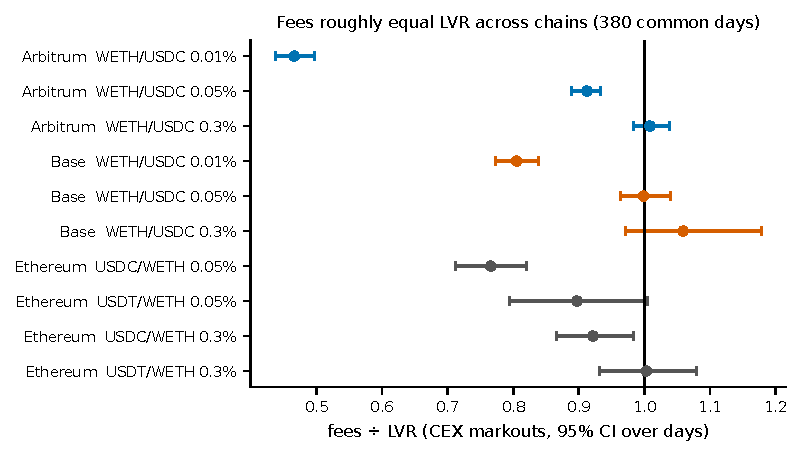
\includegraphics[width=\linewidth]{fig6_fees_vs_lvr.pdf}\end{minipage}\hfill
\begin{minipage}{.49\linewidth}\centering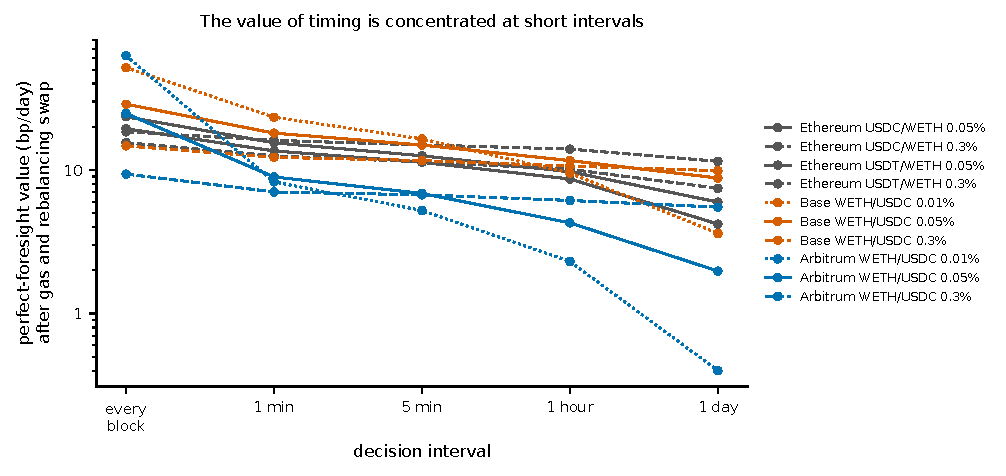
\includegraphics[width=\linewidth]{fig7_timing_ceiling.pdf}\end{minipage}
\caption{Left: fees divided by LVR (CEX markouts 12 seconds after the swap's block) over 380 common days, with 95\% confidence intervals over days. Right: perfect-foresight value of entering and leaving a 2\%-wide, \$100,000 position, by decision interval, after gas (\$15 on Ethereum, \$0.10 on layer 2s) and the swap needed to rebalance.}
\label{fig:fees}
\end{figure}

\paragraph{The value of timing.} An upper bound on that value comes from a perfect-foresight policy that holds liquidity only in intervals where fees exceed LVR, paying gas and a rebalancing swap at each entry. The bound falls steeply with the decision interval (Figure~\ref{fig:fees}, right). For Ethereum USDC/WETH 0.05\%, where always staying in range loses 27 bp per day on this position, perfect timing would earn 23.5 bp per day at block resolution, 15.5 at one-minute intervals, 9.7 hourly and 6.0 daily. On Arbitrum's 0.01\% pool it falls from 62.6 per block to 0.4 per day. Most of the attainable value therefore lies at horizons of minutes and below, which is the regime where an event-level simulator, rather than a horizon-level price forecaster, is the natural tool. We do not claim that our model captures this value: no forecast-driven policy we tested beat its costs. % CHECK: this refers to the earlier gating experiments (gate_experiment.py), not reported in detail here.

% ===================================================================== 8
\section{Limitations}\label{sec:limitations}

\begin{itemize}
\item \textbf{Single-pool histories.} The model sees one pool's history; cross-pool and centralised-exchange information, which drives arbitrage flow, is absent.
\item \textbf{Small-position overlay.} Simulated paths do not react to the evaluated LP's own liquidity.
\item \textbf{Scope.} Training uses ten Ethereum pools; only two pools are held out.
\item \textbf{Remaining failures.} Skew is not directionally informative; swap-size tails are still heavier than real; 15\% of held-out paths still collapse (5\% in reality); volatility clustering is too strong; JIT is too rare, too large and too sticky.
\item \textbf{Baselines.} On the seen-pool test period, the recent-history forecaster is better at 512 events; on held-out validation pools it is slightly better at 128 and 512 events.
\end{itemize}

% ===================================================================== 9
\section{Conclusion}

Learning only the stochastic part of AMM order flow, and computing the rest exactly, gives a simulator whose every state is valid and inspectable. Exact mechanics also turn out to be a source of information: conditioning on the pool's liquidity profile, available for free during simulation, is what makes long rollouts work on unseen pools, even though it slightly worsens next-event likelihood. That divergence is the clearest lesson of this study: for simulators, one-step likelihood is the wrong target on its own. Multi-pool simulation conditioned on external prices is the natural next step.

\paragraph{Code and data.} Code (Apache-2.0) and the reconciled dataset (CC BY 4.0) are available at \url{https://github.com/Claybarn/DEX-Net}. % CHECK: repository is private until release.

\bibliographystyle{plainnat}
\bibliography{refs}

% ===================================================================== A
\appendix
\section{Supplementary results}

\begin{table}[t]
\centering
\small
\caption{Macro next-event NLL by model component (nats per event of that type; Clock, Event type and Joint per event), mean over 3 seeds.}
\label{tab:nll_by_head}
\begin{tabular}{lrrrr}
\toprule
Component & Ref. (seen) & Depth (seen) & Ref. (held out) & Depth (held out) \\
\midrule
Clock & 2.421 & 2.422 & 4.451 & 4.456 \\
Event type & 0.667 & 0.669 & 0.667 & 0.668 \\
Sell size & 2.003 & 2.004 & 2.298 & 2.317 \\
Buy size & 2.253 & 2.263 & 2.030 & 2.035 \\
Mint lower & 4.129 & 4.124 & 3.459 & 3.474 \\
Mint width & 3.223 & 3.216 & 1.945 & 1.935 \\
Mint amount & 2.630 & 2.623 & 2.226 & 2.263 \\
Burn lower & 3.468 & 3.453 & 2.545 & 2.545 \\
Burn width & 0.877 & 0.876 & 0.651 & 0.651 \\
Burn amount & -0.480 & -0.471 & -0.697 & -0.646 \\
Joint & 5.534 & 5.542 & 7.649 & 7.667 \\
\bottomrule
\end{tabular}
\end{table}


\begin{figure}[h]
\centering
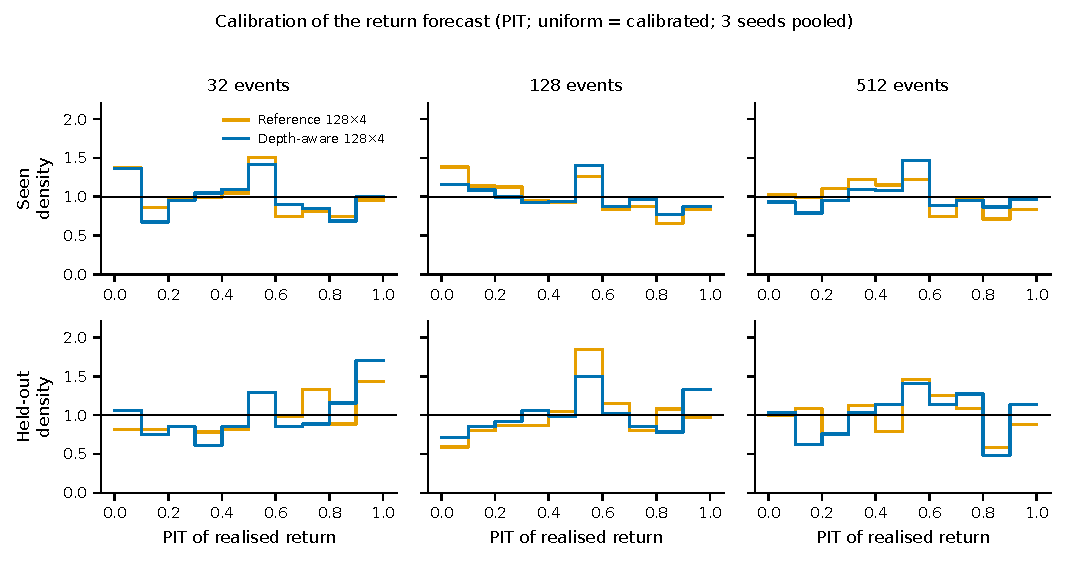
\includegraphics[width=\linewidth]{figS1_pit.pdf}
\caption{Probability integral transform (PIT) of the realised return under each model's forecast, pooled over three seeds; a calibrated forecast gives a uniform histogram (density 1).}
\label{fig:pit}
\end{figure}

\section{Reproduction}
\sloppy
The final runs are defined by \texttt{paper/final/matrix.json} and trained with \texttt{scripts/run\_matrix.py}; evaluation is \texttt{paper/final/evaluate.sh}, and the JIT and point-process analyses are \texttt{scripts/jit\_analysis.py} and \texttt{scripts/hawkes\_baseline.py}. Figures and tables are generated from the result files by \texttt{paper/figures/make\_figures.py} and \texttt{paper/tables/make\_tables.py}.

\end{document}
